%%%%%%%%%%%%%%%%%%%%%%%%%%%%%%%%%%%%%%%%%%%%%%%%%%%%%%%%%%%%%%%%%%%
%                                                                 %
%                            CHAPTER TWO                          %
%                                                                 %
%%%%%%%%%%%%%%%%%%%%%%%%%%%%%%%%%%%%%%%%%%%%%%%%%%%%%%%%%%%%%%%%%%%

\chapter{PREVIOUS WORK}
%\resetfootnote %this command starts footnote numbering with 1 again.

A number of instances in the literature mentioned previously uses the term versioning and provenance interchangeably.
Mayernik et al. also notice a similar phenomenon although they use the term lineage instead of versioning \cite{MatthewS.Mayernik201312-039}.
The version model introduced by Barkstrom in Figure \ref{NASALevels} to organize NASA's satellite data collection actually refers to a simplified workflow describing the provenance used to produce each level of data \cite{Barkstrom2003}.
The diagram does not compare objects from the same level since changes to contributing components are only used as an indicator for version change.
In actuality, objects have much more complicated development structures than the one dimensional lifespan indicated by the transition from Level 0 data to Level 3.
The PROV Ontology model in Figure \ref{PROVO} outlines more explicit inter-relations between data objects, and it provides a new dimension with which to consider the interactions of data objects.
More specifically, it outlines the explicit process of an agent performing an activity using an entity to produce a new entity.
In the context of the level system, an agent (either a program or individual) performs a "Produce Instantaneous Fields" activity using "L1 Data" to produce "L2 Data."
However, higher level data sets rarely use only one instance of lower level data.
Calibration values may result from daily readings collected from another data set, but the generality of the ontology allows these relationships to be explicitly expressed.
A more realistic provenance graph looks like the one in Figure \ref{ProvGraph} of an ozone indicator in which a Level 3 object results from the interrelation of multiple lower level products.
An interesting observation of note is that Tilmes remarks in 2011 \cite{TILMES2011548}, 
\begin{quotation}
	Consider the relatively common case of the calibration table, which is an input to the L1B process, changing. Even though the version of the L2 or L3 software hasn’t changed, the data files in the whole process have been affected by the change in the calibration.
\end{quotation}
which Barkstrom already observes in 2003 \cite{Barkstrom2003}
\begin{quotation}
	If scientific data production were easy, instruments would
	have stable calibrations and validation activities would discover no need for
	corrections that vary with time. Unfortunately, validation invariably shows that
	instrument calibrations drift and that algorithms need a better physical basis. Within a Data Set, we can think of a Data Set Version as a collection of files in
	a Data Set that have a homogeneous Data Production Strategy. Within a Data
	Set Version, we expect the code producing the files to be stable. We also expect
	that the algorithm input coefficients will be stable as well. The intent of data
	production is to produce data whose uncertainties are statistically similar under
	similar conditions of observation.
\end{quotation}
indicating a basic view that despite eight years in difference, the continuation of software focused versioning resulting in difficulties of data oriented collections.

\begin{figure}
	\centering
	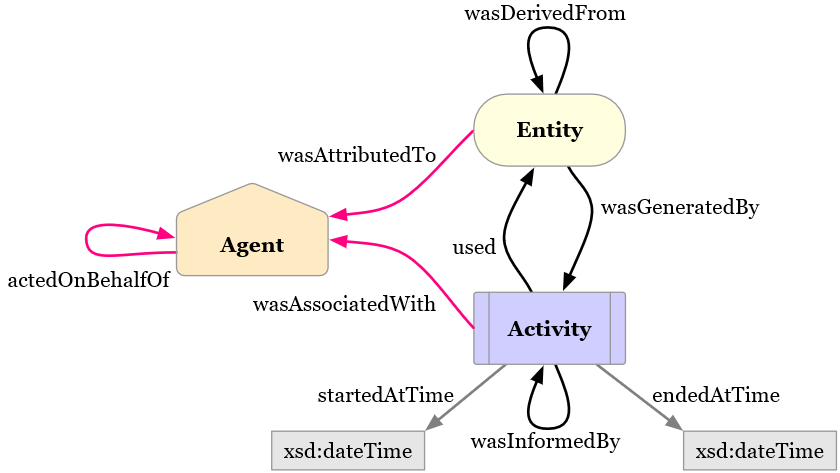
\includegraphics[scale=0.5]{figures/ProvO.png}
	\caption{Diagram of the PROV Ontology.  Figure 1 from \cite{Lebo2013}}
	\label{PROVO}
\end{figure}

\begin{figure}
	\centering
	\begin{adjustbox}{addcode={\begin{minipage}{\width}}{
					\caption{Provenance graph of a Level 3 data product, showing the inter-relations between different data products in generating the final product.  Figure 2 from \cite{TILMES2011548}}\end{minipage}},rotate=90,center}
		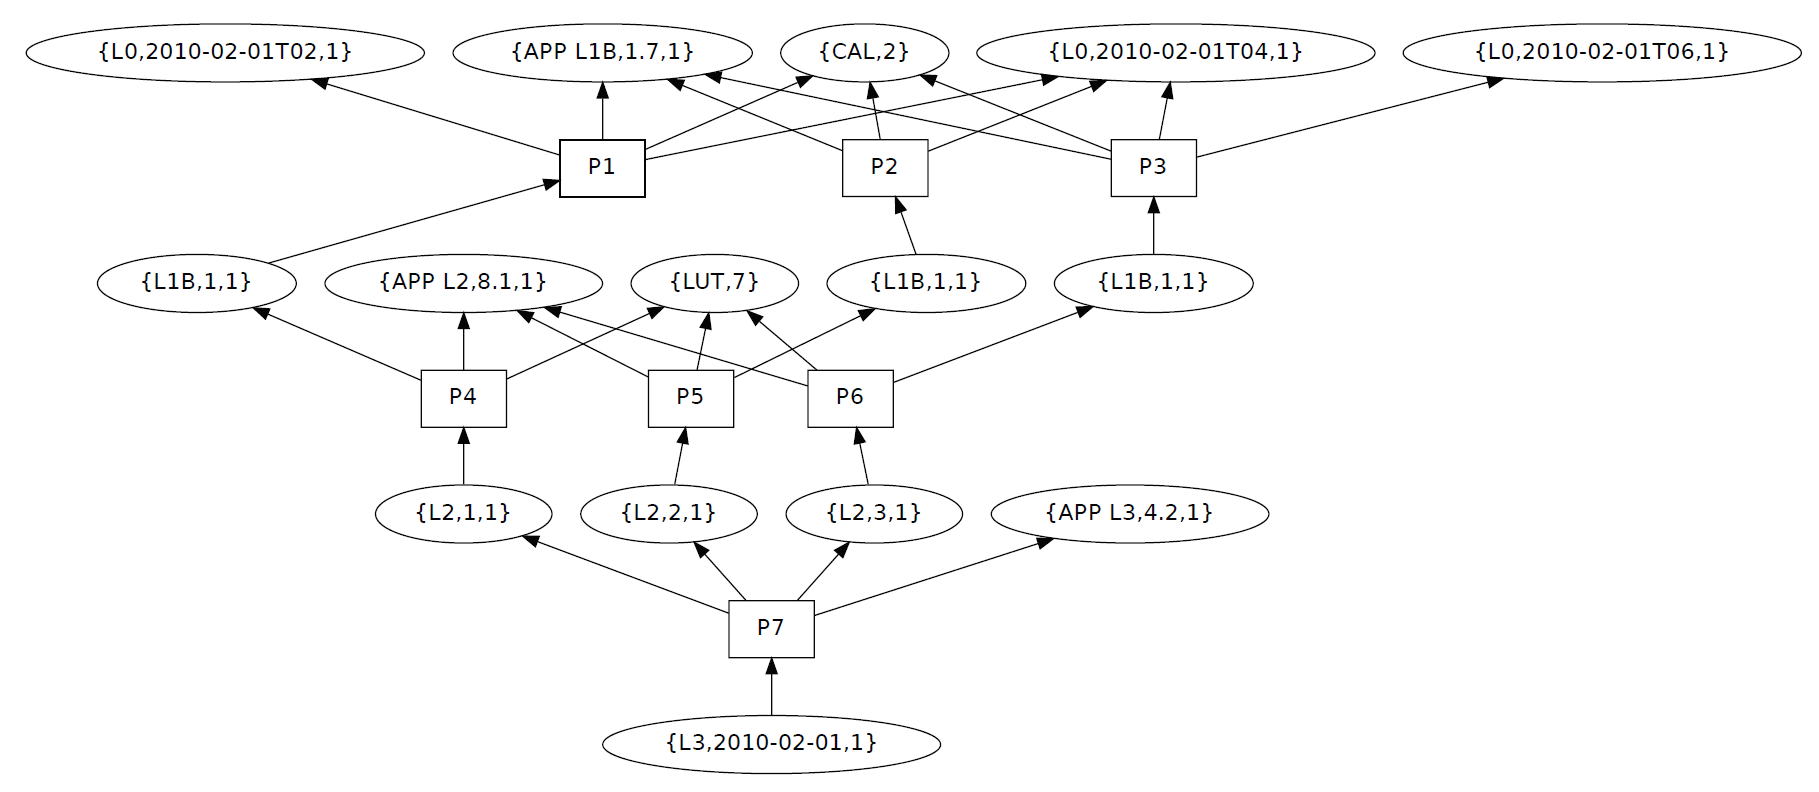
\includegraphics[scale=0.5]{figures/OzoneProvGraph.png}
	\end{adjustbox}
	\label{ProvGraph}
\end{figure}

If the level system provides a length and provenance indicates a breadth of a workflow, a version system can be considered to provide a height to a total workflow.
Referring back to the HCLS data model terminology in Figure \ref{HCLSModel}, as objects within a workflow, as in Figure \ref{ProvGraph}, change versions, the structure of the workflow as well as the Summary Description of the final object, in this case the L3 Ozone product, remains the same.
Instead, the new versions add layers like building blocks over the foundations of the original workflow structure.
Version control systems then provide the mortar linking the blocks together to give the lineage capture procedure a solid structure.
The PAV Ontology provides a means to track versioning information through linked data by introducing \textit{pav:version} to cite versions and \textit{pav:previousVersion} to link them together in order \cite{Ciccarese2013}.
It does so in comparison to the Dublin Core concept \textit{dc:isVersionOf} which records, "Changes in version imply substantive changes in content rather than differences in format" \cite{DCMI2012}.
PAV argues that a new concept becomes necessary to cover cases where new versions do not have to be substantive but can still be alternate editions of the original object.
Of note is the retrospective nature of the PAV ontology and PROV-O since it places primary emphasis on the most recent edition of an object.
Figure \ref{RCSTree}, shows how RCS stores older versions as back deltas and branches as forward differences.
The retrospective nature of back deltas results from development focus on the latest version, in this case 2.2.
However, the forward differences provide a method to migrate from version 1.3 to the front of the branch.
This characterizes the difference between a focus on data tracking, like that performed by provenance, to data migration, which users must undergo in order to consume the latest version.
Mayernik et al. also find that, "Prospective records document a process that must be followed to generate a given class of products whereas retrospective records document a process that has already been executed" \cite{MatthewS.Mayernik201312-039}.
Retrospective provenance and versioning provides the ability to ensure data trustability and data quality among resources.
However, researchers must follow a prospective versioning record in order to keep their research up to date.


To bring the discussion to an actual application, the GCMD released version 8.4 of their keywords, adding a slew of new values and modifying a select few \cite{Stevens2016}.
At the time of release, many data repositories can be currently assumed to be using the previous or older versions of the keywords.
As the taxonomy is not a class-based ontology, changes to the keywords have significant implications to the semantics of a data set described by those keywords.
A data producer wishing to expose their data sets using the new version of the GCMD Keywords must use a prospective method to translate their current descriptions to the new version.
By comparison, the GCMD would use a retrospective measure to record the changes made to their keywords.
PAV would not be able to address the prospective problem as a result of it is, "a lightweight vocabulary, for capturing “just enough” descriptions essential for web resources representing digitized knowledge" \cite{Ciccarese2013}.
A detailed transition from GCMD Keywords 8.3 to 8.4 would significantly undermine the lightweight nature of the vocabulary.
GCMD does provide a short summary of changes made in a version, but this would come in the form of text rather than structured data.

\section{Provenance}

Early attempts at encoding provenance data into semantic models include the development of the Proof Markup Language \cite{daSilva2006381}.
While this was originally developed to express inference reasoning through traceable graph relations, the model can also be used to express the provenance of products using the same transitions.
The power is that it is able to use terms defined on the Semantic Web to construct inferences.
This early demonstration of the ability for web based semantic technologies also expresses complex relations in a way that can be reasoned over and computed.
It then allows for autonomous solutions to understanding change as data freshness begins playing a significant role in successful system function \cite{Bouzeghoub:2004:FAD:1012453.1012464}.

Not long after began the development of the Open Provenance Model (OPM) \cite{moreau2008open}.
Driven by the uncertain needs and sometimes conflicting conventions of different scientific domains, the model sought to find a method to standardized the way in which provenance data is captured while also keeping the specification open to accommodate current data sets through the change.
In an experimental case, the model has been applied to sensor networks to automate and unify their provenance capture even as they grow \cite{5478496}.
To aid in the adoption of the OPM, the framework Karma2 was developed to assist integrating provenance capture into scientific workflows \cite{simmhan2010karma2}.
It reduces the amount of modifications required to adopt the OPM through web services and, more importantly, integrates into scientific workflows.
With the magnitude of data collection endeavors, it is no longer feasible for scientists to stay close to the data and must take a more abstract view of their data collection activities.
Scientific workflows provides this high level view of complex data collection, curation, and analysis \cite{Casati1996}.
The value then of integrating provenance capture and workflow design is that lineage planning can then take place at a high level of scientific work.
This gives insight into how different parts of the workflow fit together and how new exploratory expansions may occur.

Following the OPM, PROV is a W3C recommendation that deliniates a method to express data provenance with semantic technologies that has been accepted as a World Wide Web Consortium (W3C) Recommendation \cite{Gil2013} \cite{Gil2013a} \cite{Groth2013}.
The recommendation uses a conceptual model relating activities, agents, and entities together to describe data production lineage \cite{Moreau2013c} \cite{Nies2013} \cite{Nies2013a}.
Intended as a high level abstraction, it describes data as entities that are generated by activities enacted by agents.
This basic relationship is very powerful in its ability to describe data production activities.
The expression of the conceptual model occurs through the PROV Ontology (PROV-O), which can be conveyed through various resource description languages \cite{Lebo2013} \cite{Hua2013} \cite{Klyne2013}.
The ontology is further formalized into a functional notation for easier human consumption \cite{Moreau2013b} \cite{Cheney2013a}.
One particular strength that has contributed to the adoption of PROV is its ability to link into other ontlogies, making it easier for existing semantically enriched data sets to adopt PROV \cite{Miles2013} \cite{Moreau2013}.
Like the OPM, a framework has also been developed to alleviate workflow integration through Komadu \cite{Suriarachchi_2015}.
The framework improves over its predecessor, Karma, by no longer utilizing global context identifiers that were no necessarily shared throughout the workflow.

The PROV Ontology provides four different concepts that begin to encapsulate the provenance relationship between data versions.  The ontology defines a prov:Generation as "the completion of production of a new entity by an activity," \cite{Lebo2013}.  This means that the generation must result from a prov:Activity.  In versioning, activities play a much less active role since changes become exposed from comparing like objects.  It creates a relationship between an entity and an activity, but such a relationship may lead to an implication that a change in the activity resulted in changes in the resulting version.  Changes could also result from modifications in the input data, leading to an entirely new generating activity rather than a modified one.  Prov:Invalidation likewise makes a similar connection between activities and entities.  This means that PROV-O does not have the direct means to communicate the addition and invalidation relationships which exist in a versioning context.  Since versioning relationships result from state-based effects between version entities, a more contextually appropriate relationship would connect two entities together.  The property prov:Derivation does relate together two entities and the ontology defines it as, "a transformation of an entity into another, an update of an entity resulting in a new one, or the construction of a new entity based on a pre-existing entity. " \cite{Lebo2013}.  In the case of the MBVL dataset, none of these three assertions hold true.  The four versions are being simultaneously considered so one is not being transformed into another as would a sequential set of versions.  Additionally, since we do not know which version is the best, we cannot consider any version an update of the others.  Finally, no entity pre-existed as the data sets resulted from an ongoing analysis and further steps have not been developed.

PROV has played a significant contribution in maintaining the quality and reproducibility of datasets and reporting in the National Climate Assessment (NCA) \cite{Ma2014191}.
This implication signifies that there is an increased likelihood of adoption through other scientific fields as a result of this reporting.
The Global Change Information System, which houses the data used to generate the NCA, uses PROV to meticulously track the generation of its artifacts and results as they are used in the report \cite{Tilmes2012}.
This means that not only does the data have a traceable lineage to verify quality, but the content of documents can have the same verifiability \cite{Ma2014}.

\section{Provenance Distance}

Understanding provenance and workflows only provide only a portion of the view into a data set's lineage landscape.
The workflow provides an understanding of how a data set fits into the bigger picture of data analysis and the provenance gives a method to reproduce the data set for data quality purposes.
As such, workflow and provenance describe data sets in a very flat and static manner, allowing for prospective reasoning as to how it may respond to changes made by the data producers.
However, this places the burden of determining the magnitude of change in quality, as changes in provenance mean changes in quality, on the data producer.
Consider again that data quality is subjective with respect to the data consumer's usage, and the difficulty in determining the significance of a new version becomes apparent.
With increasing complexity, data workflows have developed in such a way that even subtle changes have serious implications for other parts of the workflow \cite{TILMES2011548}.
The responsibility of determining and communicating the magnitude of data alterations falls to versioning systems.

A very rudimentary way to communicate change distance uses the version number of the data set.
Returning to discussing the dot-decimal notation often used to identify versions, version numbering follows a hierarchical method of systematically counting the releases made to a data set or system based on the perceived magnitude of the change.
The problem lies with identifying the extent of perturbations performed upon the data set.
The primary function of the number is to indicate compatibility not changes.
Therefore, a release can result from five perturbations or fifty modifications.
These cases become challenging since some users will experience larger perturbations resulting from a change than others.
As a result, using fewer well-established categories avoids this problem, but it loses many details in resolution of the extent to which the data set may change.
In addition, there is no standardization as to what each of the numerals used in a version number represents, and this significantly hinders interoperability between information systems.
Data managers will often discuss whether data sets are qualitatively different enough to warrant incrementing one of the version numerals.
While the dot-decimal method is easy to implement and use, its broad categorization severely impairs its ability to express version information beyond a basic functional extent.

Another approach is following the provenance of two data sets and identifying  differences between the lineages of the two data sets.
The total difference between the data is known as their provenance distance.
This distance measure is very new as the availability of computable provenance has been developed fairly recent.
One endeavor to compute over provenance has shown a marked ability to predict disk usage based on the lineage of a data object \cite{dai2014provenance}.
Efforts have also been made to summarize provenance representations to improve consumption \cite{Ainy:2015:ASD:2806416.2806429}.
While the ability to compute over provenance data has been demonstrated, the comparison of two provenance graphs has yet to be widely studied.

Using PROV to represent provenance data in a semantic model produces an acyclic directed graph with labeled nodes.
As a result, the provenance distance problem reduces to the similarity measurement problem.
When measuring similarity, algorithms determine how far two graphs are from being isomorphic \cite{Cao2013}.
General graphs have similar complexity to determine similarity, but node labeling simplifies this process by providing a method to match nodes together.
Other methods also exist to determine similarity under different conditions such as edits necessary to transform one graph into another  \cite{Gao2010}.
Some methods focus primarily on edge changes \cite{Goddard:1996:DGU:246962.246972}.
In Figure \ref{GraphEdit}, the left graph transforms through a move of edge 1 and a rotation of edge 4, resulting in an edit distance of two.
Such changes in a provenance graph would demonstrate a change in dependencies between objects used to generate a final product of note.
A difference in provenance distance would then provide context for differences between conclusions.
Similar results from data with small provenance distance would ensure reproducibility, while large distances signals reinforcing confirmation of a result.
However, differences can always be expected when considering different versions with more detailed comparisons required to determine the implications of changes made to a data set as a result of a provenance change.
Meanwhile, when results disagree, a small provenance distance indicates that findings may not be reproducible.
This kind of analysis resembles comparison measures employed in determining semantic similarity \cite{Hliaoutakis06informationretrieval}.
The main difference lies in semantic similarity comparing the distance between two concepts within a graph as opposed to the distances between the graphs themselves.
However, it does reveal that using semantic graphs can have incredible impact in extracting implied relations between data they store.

\begin{figure}
	\centering
	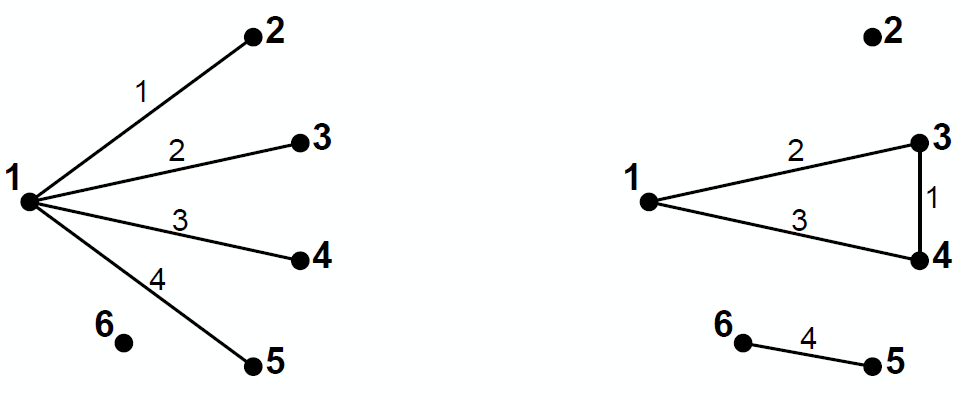
\includegraphics[scale=0.40]{figures/GraphEdit.png}
	\caption{The labeled graph on the left transforms into the right graph under two edge edits. Figure 2 from \cite{Goddard:1996:DGU:246962.246972}}
	\label{GraphEdit}
\end{figure}

There already exist methods which compare workflows based on quality criteria that leverages provenance to bound quality of service \cite{2015:CAA:2778374.2778504}.
However, these procedures focus primarily on quick retrieval and efficient storage instead of leveraging the latent information accessed by reasoning across data set versions \cite{tan2004research}.
The distance measures previously mentioned rely solely on provenance graphs to compute results, but this is obviously insufficient.
When considering the provenance of a data object, methods only consider the activities and entities that took an active role in the production of it.
A new version of an object has a familial relationship with its previous versions, but in most cases, they do not take an active role in its generation.
For this reason, detailed change information falls outside of provenance's scope and it can be seen in PROV using a single relation to link different versions of a data object.
Without detailed change information, determining the difference between two data objects in a metric beyond broad strokes becomes difficult if not impossible.

This is not to say that provenance becomes useless in computing change distance, but it largely serves as an indicator than a measure.
If there is any difference in provenance, then something must have changed.
For example, if workflow uses a new script to generate a data set, changes can be expected in this new data set.
However, what this script does differently than the old one requires a more detailed understanding and description than lineage can provide  \cite{Bose:2005:LRS:1057977.1057978}.
Additionally, if no changes were made to the script, but new data was produced, it likely indicates that some inputs have changed.
The ramifications for the resulting data set will be difficult to determine without understanding how the original inputs have changed.
Only knowing that they have changes is insufficient.
Being able to understand the extent that modifications to data or workflows impact the results greatly improve a producer's ability to generate high quality data.

\section{Spreadsheets}

In this project, spreadsheets were chosen for study as they resemble text-like data objects while still maintaining a level of complexities.
Though not as well encapsulated as other data format types such as the Hierarchical Data Format (HDF) or Network Common Data Form (NetCDF), spreadsheets provide many helpful tools that scientist favor for quick data storage and distribution over comma separated values (CSV).
There also exists other document-like formats that are not discussed in this paper such as eXtensible Markup Language (XML).
The initial work was done with the "Noble gas isotope abundances in terrestrial fluids" workbook (Noble Gas) \cite{Polyak2015}.
The "Paragenetic Mode for Copper Minerals" workbook (Copper Data) was used to give better insight into data changes due to collaboration with the data set's author \cite{Morrison2016}.

The Noble Gas data set was initially published on June 11, 2013 and then released a second version on March 8, 2015.
Many significant changes were made to the data set between the two versions, which makes this data set particularly challenging to version.
The physical structure of the data set changed from eight separate Excel spreadsheets to a single spreadsheet.
The second version also trimmed 195 columns to 54 columns in the second release.
In addition, many new locations were surveyed and added to the second release.
Documentation accompanied the data set explaining different components of the spreadsheet and its usage, but it included no versioning information.
This lack of versioning or transitioning information indicates a focus on data usage rather than data maturation, which is not a particularly bad approach.
It makes logical sense to simply download the latest data set when it becomes available and not worry about the format of the invalidated data set.
This approach convenient for new users of the data as the cost to consumer the new version of the data is the same cost they would have spent to acquire the data in the first place.
However, users of the old data are disproportionately effected by the change in versions since old code and workflows may need to be updated to accommodate the changes in addition to the cost of consuming the architecture of the old data set.
In this case, users would need to read the documentation to understand whether 182 from the June data set is still available in the March data and, if it is, in which column it resides in the March spreadsheet.
This brings to light the additional concern for the Noble Gas data that the documentation is not easily machine consumable, meaning that all mapping activities will need to be performed manually.
Not only is this approach time consuming, but it also does not scale well into larger data sets.

The Copper data set was acquired during the process of a workshop to generate new methods of visualizing mineralogy data, initially on June 8, 2016.
The process entailed trying various orders and organization for the data and results in various new versions of the data that depend on varying filtering requirements, acquired on August 21, 2016.
Unlike the Noble Gas data set, the Copper Data had no accompanying documentation, since the primary consumers of the data at the workshop were also mineralogy experts.
However, this data set had more stable characteristics including physical and logical structure.
Only two columns were removed from the transition to the second version, but sixteen new columns were added to the data collection.
It also demonstrates a change in orientation with respect to data usage since the previous data set was designed to be distributed for general usage and discovery.
In this case, the structure and organization of the data within the set was driven for a specific purpose in the development of more expressive visualizations.
As a result, versioning information is driven by developmental needs instead of the other way around with versioning information bridging the gap between software migrations.

The data files from both data sets can easily be tracked using standard version management services such as GIT or SVN.
Likewise, there exist comparison tools like Spreadsheet Compare from Microsoft Corporation that can generate diff-like outputs for each of the data sets.
In conjunction with commit logs, the comparison outputs provide a basic versioning methodology that describes the data set's evolution.
However, these applications rely on human attention and interaction to operate, and with larger data sets, proper documentation becomes difficult to maintain.
With the Copper Data, the demand for new versions of the spreadsheets exceeded the time necessary to document version history as a result of rapid product evolution during the workshop.
In consequence, the process to manually commit and annotate changed data impairs the natural progression of scientific development.

\section{Database Systems}

Databases remain the most relied upon technology for storing and searching large quantities of data rapidly.
While the dynamic combination of tables means that data bases remain flexible enough to represent complex objects, it also means that they represent a much more complicated case for attribution.
Since tables may be combined in different ways to answer complex queries, indexes do not remain constant across requests to the database.
The approaches to database versioning typically focus on ensuring the reproducibility of queries to the database.
This can often be difficult as with spreadsheets since changes to the content or structure can result in different solutions from the database for the same query even using time stamps.
For example, consider the query to select all columns of row A from a database on March 1st, then the database undergoes a schema change to add a new column to the table on April 1st.
A subsequent request for all columns of row A would include the new column which does not represent the response on March 1st.
In addition, even if the data is timestamped, the time signature is associated with the row and not the schema, meaning that the query may still return row A with the new column with a NULL value, depending on the distribution.
The query, not the data, would need to be modified to exclude the new column.

This presents as a challenge because unlike data files and spreadsheets, databases are generally not instanced.
Databases often store massive quantities of data and replication of that data to archive snapshots or distribution frequently proves too costly to be feasible.
Instead, interaction with the database occurs from a centralized source through transactions.
Various methods have been studied to manage changes within these systems focusing primarily on schema versioning, emphasizing data's structural component \cite{roddick1996model}.
This provides a method to enact a transactional rollback on the database to execute queries in an environment reminiscent of the original execution.
The framework of the resulting database environment can become quite complicated as a result of the complexity of the tables representing intricate data objects \cite{Klahold:1986:GMV:645913.671314}.
This results from the need to manage the time instances of realization, storage, and validity.
The datum becomes realized at collection, then stored upon entry into the database, and finally valid until the present or new data replaces it.
More recently, new methods have been developed to adjust to the enormous quantities of data populating modern databases, focusing on query citation rather than data citation \cite{Proell2013} \cite{DBLP:conf/data/2013}.
Citation by query avoids the complexities involved with referencing data that can grow and move.
However, this method relies on the existence of a versioning system for data.
This method also recognizes that modifying queries to operate on the current state of the database may often be easier than rolling back transactions or schema to reproduce the results of a query \cite{proellBigData}.
As a result, to versioning a database system may be more feasible as data size increases by applying methods to the query results and not to the data.

The RRUFF Database is "an integrated database of Raman spectra, X-ray diffraction and chemistry data for minerals" \cite{Lafuente}.
It features a web accessible change log using the transactional log generated by the database software\footnote{\url{http://rruff.info/index.php/r=rruff_log_display}}.
As the records in specific tables change, the log reports these changes, supplying persistent access to the modifications made to the RRUFF data.
The approach to this alteration information highlights the always on-line approach to modern databases where changes to the data do not constitute a new database.
The log demonstrates strong versioning characteristics with not only a breakdown of the change components, but also a commentary on the motivation for the difference.
In addition, its HTML structure allows automated web crawlers to systematically consume the version information.
With the integration of web ontologies, the change log would also be intelligible to automated agents.

\section{Ontologies}

On-line ontologies are a different way of storing data than relational databases that has found significant traction within Semantic Web applications.
They form graphs, relating a vocabulary of terms and relationships together to model complex interactions within an application's domain.
Since the ontology is represented as a graph, it has more expressiveness than relational databases.
The objects no longer need to share uniform structure and fields when entered into the database.
Ontologies improve interoperability between scientific data sets by allowing differing data to share a common vocabulary and be comparable.
Like other data, ontologies change regularly as definitions and relationships update to better represent their source material \cite{Ochs:2015:SVS:2826733.2826866}.
As a connected graph, they easily lend themselves to providing mappings between changes and versions within the ontology.
New transitions would be represented as a simple link between new and old concepts.
This is particularly important on the Semantic Web since most reasoning and interactions are handled automatically by underlying services.
Ontologies, thus, benefit the most when providing both forward and backward mapping as it allows more up to date systems to interact with entities that haven't migrated yet \cite{Klein01ontologyversioning}.
Incomplete mappings, where transitions exclude either forward or exclude backward mappings, retain value as backward mappings inform traceability and forward mappings communicate advances in the domain.
However, the uncertain landscape of web services means that full ontology mappings prove invaluable to making data inter-operable.
Advances in ontology change detection have made tools which automatically generate mappings between versions of an ontology available \cite{Hartung201315}.
However, in this project, the focus remains on improving the description of these mappings to provide not only descriptions but also explanations for the transition.


%%% Local Variables:
%%% mode: latex
%%% TeX-master: t
%%% End:
